\chapter{Marco Conceptual}

En este capítulo se describen los conceptos necesarios para que el lector se pueda familiarizar con mayor facilidad con los conceptos usados en el resto del informe, describiendo lo que se entiende por los conceptos usados en términos de redes sociales y conceptos asociados al desarrollo de la solución.\\

En caso de así preferirlo, el lector puede saltar las secciones que estime convenientes dentro de este capítulo, en caso de dominar los conceptos y usar este capítulo como referencia en caso de necesitarlo.

\section{Conceptos de Redes Sociales} % (fold)
\label{sec:conceptos_de_redes_sociales}

\subsection{Definiciones} % (fold)
\label{sub:definiciones}

% subsection definiciones (end)
% section conceptos_de_redes_sociales (end)

\section{Conceptos de Desarrollo} % (fold)
\label{sec:conceptos_de_desarrollo}

A continuación se explican los términos en lo que a desarrollo que se refiere que tienen relación con el trabajo realizado en esta memoria.

\subsection{Modelo MVC} % (fold)
\label{sub:modelo_mvc}
El modelo MVC (Modelo, Vista, Controlador), consiste en un modelo para separar la lógica de una aplicación agrupándola en clases u otras unidades modulares, de acuerdo con la responsabilidad que estos módulos cumplan dentro de un sistema. A modo de ejemplo, a fin de ilustrar este concepto, se puede dar un caso de una aplicación que registre compras en un sistema de tienda online, un ejemplo de los módulos asociados a compras en MVC puede ser el siguiente:

% TODO: insertar imagen model MVC aquí
\begin{figure}[!h]
  \centering
  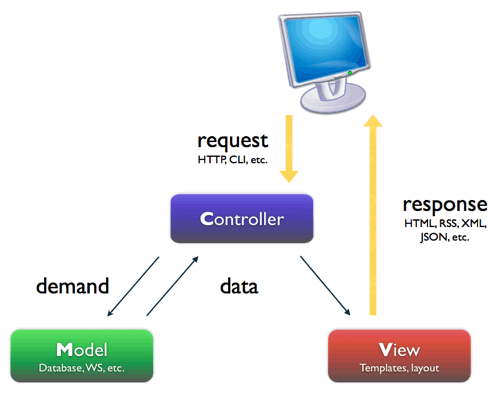
\includegraphics[scale=.5]{images/mvc.png}
  \caption{Modelo MVC}
  \label{modelomvc}
\end{figure}

\begin{itemize}
  \item \textbf{Modelo}: el modelo corresponde a una clase \texttt{Compra} que contiene toda la lógica de negocio asociada a las compras, que además se asocia directamente a como se almacena una compra en la base de datos.
  \item \textbf{Vista}: un ejemplo de vista para una compra, puede ser una interfaz \texttt{HTML} en la cual el cliente efectúe operaciones sobre la compra, por ejemplo agregar productos, cabe destacar que la vista no ejecuta las acciones, sólo se encarga de recibirlas y enviarlas al último componente del modelo MVC, el controlador.
  \item \textbf{Controlador}: de acuerdo a lo recién expresado, el controlador es el encargado de coordinar uno o más modelos para ejecutar las acciones capturadas en la vista. En el caso de la compra, el controlador es quien efectivamente procesaría el pago de la misma.
\end{itemize}
% subsection modelo_mvc (end)

\subsection{Frameworks de Desarollo} % (fold)
\label{sub:frameworks_de_desarollo}
Un framework de desarrollo define un marco en el cual desarrollar una aplicación, el cual provee una gran cantidad de funcionalidad común lista de manera de no desarrollar un proyecto desde cero, pero además de sólo funcionalidad, provee de una estructura lógica con la cual se escribe el código, que está influida por muchas otras personas que han usado el framework en aplicaciones reales.

\subsubsection{Frameworks Server Side} % (fold)
\label{ssub:frameworks_server_side}
Dentro de los frameworks de desarrollo web existe una categoría llamada \emph{Sever Side}, la cual consiste en que el código de la aplicación corre desde un servidor en internet, lo que permite que si la computación es común para muchos clientes, los resultados de esa computación pueden ser usados múltiples veces.\\

Ejemplos actuales de esta categoría de frameworks son: \texttt{Ruby on Rails}, \texttt{Sinatra} que utilizan el lenguaje \texttt{Ruby}; \texttt{Django}, \texttt{Pylons} para \texttt{Python}; \texttt{Spring} para \texttt{Java} y \texttt{CakePHP} para PHP entre otros.
% subsubsection frameworks_server_side (end)

\subsubsection{Frameworks Client Side} % (fold)
\label{ssub:frameworks_client_side}
En el último tiempo, surgió una nueva categoría de frameworks de desarrollo web llamada \emph{Client Side}, en la cual el código de la aplicación se ejecuta en el computador del usuario de la aplicación, ahorrando recursos necesarios en un servidor, además de ahorrar el tiempo de latencia entre el cómputo de una respuesta y su transmisión al equipo del usuario.\\

Comunmente estos frameworks son escritos para ser usados con el lenguaje \texttt{Javascript}, pues posee la propiedad que todos los navegadores web implementan un motor de \texttt{Javascript} y por lo tanto el usuario no necesita instalar nada más. Ejemplos de frameworks client side son: \texttt{AngularJS}, \texttt{EmberJS}, \texttt{Meteor} y alternativamente \texttt{BackboneJS} que es una librería más que un framework.
% subsubsection frameworks_client_side (end)

% TODO: poner referencias a los sitios de todos estos frameworks

% subsection frameworks_de_desarollo (end)

% section conceptos_de_desarrollo (end)

% ### 2.2 Conceptos de Desarrollo
% #### 2.2.1 Desarrollo Front-End
% #### 2.2.2 Desarrollo Back-End
% #### 2.2.3 El Modelo MVC
% #### 2.2.4 Frameworks de Desarrollo
% ##### 2.2.4.1. Server Side
% ##### 2.2.4.2. Clien Side
% #### 2.2.5. HTML5
% ##### 2.2.5.1 SVG, Gráficos Vectoriales en la Web